\documentclass[dvipdfmx]{ampbt}
%% compile: platex thesis.tex && bibtex thesis && platex thesis.tex && platex thesis.tex && dvipdfmx thesis.dvi

%% クラスオプション:
%% chapter:   \chapterコマンドを使用可能にする(jsbook (report) を使う).
%% duplexing: 両面印刷用の PDF を出力する.
%% その他 jsclasses に指定可能なオプションが指定できます(そのまま渡される).

%% 報告書の題目 %%%%%%%%%%%%%%%%%%%%%%%%%%%%%%%%%%%%%%%%%%%%%%%%%%%%%%%%%%%%%%%%%
\title{Friend-to-friendネットワークにおける} % 題目1行目
      {効率的な分散ルーティング}                         % 題目2行目
      {}                                         % 題目3行目
%% 指導教員 %%%%%%%%%%%%%%%%%%%%%%%%%%%%%%%%%%%%%%%%%%%%%%%%%%%%%%%%%%%%%%%%%%%%%
\supervisors{宮崎修次}{講師}    % 指導教員1人目 {氏名}{職名}
            {}{}    % 指導教員2人目 {氏名}{職名}
            {}{}                % 指導教員3人目 {氏名}{職名}
%% 入学年月 %%%%%%%%%%%%%%%%%%%%%%%%%%%%%%%%%%%%%%%%%%%%%%%%%%%%%%%%%%%%%%%%%%%%%
\entrancedate{24}{4}            % {年(平成)}{月}
%% 著者氏名 %%%%%%%%%%%%%%%%%%%%%%%%%%%%%%%%%%%%%%%%%%%%%%%%%%%%%%%%%%%%%%%%%%%%%
\author{高橋}{彰}             % {姓}{名}
%% 提出日 %%%%%%%%%%%%%%%%%%%%%%%%%%%%%%%%%%%%%%%%%%%%%%%%%%%%%%%%%%%%%%%%%%%%%%%
\submissiondate{29}{1}{XX}      % {年(平成)}{月}{日}
%% 提出年度 %%%%%%%%%%%%%%%%%%%%%%%%%%%%%%%%%%%%%%%%%%%%%%%%%%%%%%%%%%%%%%%%%%%%%
\submissionjay{28}              % {年度(平成)}
%% 摘要 %%%%%%%%%%%%%%%%%%%%%%%%%%%%%%%%%%%%%%%%%%%%%%%%%%%%%%%%%%%%%%%%%%%%%%%%%
\abstract{%
  本研究では, ネットワークトポロジーのスモール・ワールド性を利用し, 効率的かつ非中央集権的なルーティングを実現するための手法を提起する. 
}
%% パッケージの読み込みや自分用のマクロの定義 %%%%%%%%%%%%%%%%%%%%%%%%%%%%%%%%%%%
\usepackage{amsmath,amssymb, amsthm}
\usepackage{enumitem}
\usepackage{subfigure}
\usepackage{bm}
\usepackage{type1cm}
\usepackage{ascmac} % for box
\usepackage{hyperref}
\usepackage{url}
\usepackage[xindy]{glossaries}
\usepackage{algorithm}
\usepackage{algpseudocode}
\usepackage[justification=centering]{caption}
%\usepackage{algorithm2e}
\parindent = 0pt
\makeatletter
\makeatother
\newcommand{\argmax}{\mathop{\rm arg~max}\limits}
\newcommand{\argmin}{\mathop{\rm arg~min}\limits}
\newcommand{\rme}{\mathrm{e}}

%% term list
\makeglossaries
\newacronym{f2f}{F2F}{Friend-to-friend}
\newacronym{wot}{WoT}{Web of Trust}
\newglossaryentry{localcon}
{
    name={local contact},
    description={距離空間上に配置されたグラフにおいて最も近距離にあるノード間を接続するエッジ}
}
\newglossaryentry{darknet}
{
    name={Darknet},
    description={Friend-to-friendと同義}
}
\newglossaryentry{deadend}
{
    name={dead-end},
    description={メッセージを受け取ったノードが自分自身よりもターゲットに近い隣接ノードを持たない状態}
}
\newglossaryentry{embedding}
{
    name={埋め込み},
    description={TBD}
}
\newglossaryentry{swap}
{
    name={SWAP},
    description={TBD}
}
\newglossaryentry{id}
{
    name={ID},
    description={TBD}
}
\newglossaryentry{coord}
{
    name={座標},
    description={TBD}
}
\newglossaryentry{gremb}
{
    name={Greedy embedding},
    description={TBD}
}




%% 出力の制御 %%%%%%%%%%%%%%%%%%%%%%%%%%%%%%%%%%%%%%%%%%%%%%%%%%%%%%%%%%%%%%%%%%%

%% 本文を出力しない場合,次の行をコメントアウトして下さい.
% \outputbodyfalse

%% 末尾に表紙,背表紙を出力しない場合,次の行をコメントアウトして下さい.
% \outputcoverfalse

%% 末尾に提出用摘要を出力しない場合,次の行をコメントアウトして下さい.
% \outputabstractforsubmissionfalse

%% ampbt.cls では表紙等の作成のために geometry パッケージを使用しているため,本文
%% のレイアウトを変えるために \usepackage[...]{geometry} とすると Option clash が
%% 発生します.何らかの理由で本文のレイアウトを変更したい場合は \geometry{...} を
%% 使用して下さい.
%% また,jsclasses を使用しているため,例えば 3cm を指定したい場合は 3truecm と書
%% く必要があります.
% \geometry{hmargin=3truecm,vmargin=2truecm}

\begin{document}
\ifoutputbody
%% 中表紙,摘要,目次 %%%%%%%%%%%%%%%%%%%%%%%%%%%%%%%%%%%%%%%%%%%%%%%%%%%%%%%%%%%
\makeinsidecover                % 中表紙
\makeabstract                   % 摘要
\maketoc                        % 目次
\setcounter{page}{1}            % 本文のページ番号を1から始める
%% 本文 %%%%%%%%%%%%%%%%%%%%%%%%%%%%%%%%%%%%%%%%%%%%%%%%%%%%%%%%%%%%%%%%%%%%%%%%%
\section{序論}
近年インターネットを介したコミュニケーションまたは出版は, 我々の生活において大きな位置を占めるようになってきた. それに伴いユーザーのプライバシー保護を重視したコミュニケーションツールの実装に対する需要が非常に高まっている. その要因として, 例えば近年ではエドワード・スノーデンによって公に明らかにされたアメリカ国家安全保障局(NSA)による大規模な大衆監視が挙げられる. \newline
特定の企業や団体が中央集権的に管理する情報共有方式はこのような監視・漏洩のリスクが高いため, 非中央集権的な情報共有を実現するためのアプローチとしてP2P方式が頻繁に採用される. P2Pは中心的な管理者を持たない分散的なオーバーレイネットワークであり, 一般的なクライアント-サーバー方式と比較して負荷分散, スケーラビリティ, 匿名性, 耐障害性等の点で優れている\cite{lua2005survey}. そしてP2P方式の中でも特にピアの匿名性・プライバシー保護を重視したものはfriend-to-friend(\acrshort{f2f})\cite{bricklin2000friend}, またはDarknet\cite{clarke2010private}と呼ばれる. F2F方式においてネットワーク上の各ノードは, 信頼のおける特定ノードとのみ通信するため, Chord\cite{stoica2001chord}などの分散ハッシュテーブル(DHT)方式とは異なり, ソフトウェアによって動的にネットワーク構造を最適化することはできず, ネットワーク構造は常に現実の信頼関係ネットワークの部分グラフに対応する. そしてネットワーク上で隣接していないノード同士がデータの送受信を行うためにはいずれかのノードが「知り合いの知り合い」を辿って他方のノードに到達するための経路を探索する必要性が生じる\cite{roos2016dealing}.\newline
F2Fオーバーレイネットワークの最も代表的な実装例は, Freenet\cite{clarke2001freenet}のDarknetモード\cite{clarke2010private}であり, 基本的なプロトコルはSandberg\cite{sandberg2006distributed}が2006年に提案した手法に基づいている. Freenetでは, 信頼関係のネットワークがスモールワールド性を持つと仮定し, 単純なgreedyルーティング (各ノードは隣接ノード中, 最もターゲットに近いノードを次ノードとして選択) により, $O(\log^2 n)$のホップ数でルーティングを可能にするKleinbergのスモールワールドネットワークモデル\cite{kleinberg2000small}に基づいている. \newline
ただしFreenetには未だ様々な問題点が残っている. 第一にSandbergが提案した手法では, Kleinbergモデルが依拠している「格子上で最も近距離にいるノード同士は必ずエッジを持つ」という仮定を決定論的に満たすことができないため, Freenetの実装においてはgreedyルーティングの代わりにdistance-directed depth-first search ($D^2$-$DFS$)が採用されている. しかしこの$D^2$-$DFS$アルゴリズムが特定の条件下において$O(\log^2 n)$のホップ数を達成することができないことはRoos, Strufeらにより解析的に証明された\cite{roos2012provable} \cite{roos2016dealing}\cite{roos2016analyzing}. またFreenetでは, ノード集合$V$から座標空間$C= [0,1)$への「\gls{embedding}」(embedding) $\phi: V \to C$を生成するMetropolis-Hastingsアルゴリズムの一環としてノード同士が座標(Freenetの実装ではID)を交換する操作を反復するが, この際悪意のあるノードが虚偽のID報告を繰り返すことにより, ノードが格子上に偏在し, 結果的にルーティングの効率性が低下するというPitch black attack\cite{evans2007routing}などの深刻な脆弱性が指摘されている. よってFreenetのDarkenetモードは効率性や頑健性の面で問題点が残り, 現在もそれらを解決するための研究が続けられている. \newline
本研究では, 以上に挙げられたFreenetの問題点のうちルーティングの効率性に着目する. 今回我々はSimsek, Jensenらによって提案されたルーティングアルゴリズム, expected-value navigation (EVN)\cite{csimcsek2008navigating}をFreenetプロトコルに適用可能な形に修正することにより, スケールフリー性を持った\acrshort{f2f}ネットワークにおいて既存ルーティングアルゴリズムよりも高いパフォーマンスを発揮する$D^3$-$DFS$を提案する. また, 先行研究のシミュレーション実験においてはルーティングの成功率が向上するように実データの恣意的な改変が施されていたが, 本研究では改変を施さない実データに対するシミュレーション実験を行うことにより, 現実の\acrshort{f2f}トポロジーにより近いネットワークにおけるルーティングアルゴリズムのパフォーマンス評価を行った.

 \section{先行研究}
   \subsection{P2Pネットワーク}
   \subsection{複雑ネットワーク}
   \subsection{Kleinbergモデル} \label{sec:kleinberg}
   \subsection{Greedy embedding}
   \subsection{Freenetプロトコル: 埋め込みとルーティング} \label{sec:freenetprotocols}
   \subsection{EVN: Expected-value navigation} \label{sec:evn}
    \begin{eqnarray}
     E(l(v,t)) &=& \sum_i ip(l(v,t)=i)\nonumber \\
     &\approx& p(l(v,t)=1)  )\nonumber\\
     &=& 1- p(n_{v,t}=0)  )\nonumber\\
     &=& 1- (1 - p(v,t))^{k_v} )\nonumber\\
     &\approx& 1 - Poisson(0; k_vp(v,t)) )\nonumber\\
     &=& 1- e^{k_vp(v,t)} \label{eq:evn-basic}
    \end{eqnarray}
    よってある隣接ノード$v$が$E(l(v,t))$が最小化することは, $1/k_vp(v,t)$を最小化することと同値であるからヒューリスティック関数$f(v)$を
    \begin{eqnarray}
     f(v) = \frac{1}{k_vp(v,t)}\label{eq:evn-heuristic}
    \end{eqnarray}
    と定義すれば, 「メッセージを持つノード$u$は(\ref{eq:evn-heuristic})式で定義される$f(v)$を最小化するような隣接ノード$v \in N(u)$にメッセージをフォワードする」というシンプルなルーティングアルゴリズムにより, 隣接ノード中最もターゲットに近い可能性の高いノードを選択することができる. 

\if0
\cite{clarke2001freenet}
\cite{sandberg2006distributed}
\cite{sandberg2006evolution}
\cite{sandberg2008neighbor}
\cite{mogren2008adaptive}
\cite{evans2007routing}
\cite{clarke2010private}
\cite{schiller2011attack}
\cite{roos2012provable}
\cite{roos2013contribution}
\cite{roos2016dealing}
\cite{hofer2013greedy}
\cite{roos2016anonymous}
\cite{roos2016analyzing}
\cite{kleinberg2000small}
\cite{csimcsek2008navigating}
\cite{serrano2008self}
\cite{boguna2009navigating}
\cite{boguna2009navigability}
\cite{kleinberg2007geographic}
\cite{cvetkovski2009hyperbolic}
\cite{krioukov2010hyperbolic}
\cite{boguna2010sustaining}
\cite{papadopoulos2015network}
\cite{blasius2016efficient}
\cite{kleinberg2006complex}
\cite{huang2014navigation}
\cite{van2010graph}
\fi
\section{問題設定}
\ref{sec:freenetprotocols}節に述べた\acrshort{f2f}ネットワークにおける分散ルーティング効率を向上するための大まかな方針として (1)埋め込みアルゴリズムの改良 (2)分散ルーティングアルゴリズムの改良 の2通りを挙げることができる. 本研究では後者の方針を選択する. つまりSandbergによる\gls{swap}がgreedy embeddingでないという前提の上で, SWAP適用後のネットワークにおけるルーティング効率を改善させるための方法を模索する. \newline
その上で今回我々は\acrshort{f2f}ネットワークが持つスケールフリー性に着目し, \ref{sec:evn}節で述べた{\c{S}}im{\c{s}}ek, Jensenのヒューリスティックスを取り入れることでFreenetプロトコルにおける分散ルーティングのパフォーマンスを向上させることを試みる. つまり, 今回我々が検証する仮説は「greedy embeddingでないSWAP適用後の\acrshort{f2f}ネットワークにおいて, 単純なノード間距離に応じたヒューリスティックを用いる代わりに, 隣接ノードの次数とノード間距離を共に考慮したヒューリスティックスを用いることで, ルーティングのパフォーマンスを向上させることが可能である」とまとめることができる. 以下この仮説検証のために, $D^2$-$DFS$とEVNを統合したルーティングアルゴリズム, degree-and-distance-directed depth-first search ($D^3$-$DFS$)の提案とパフォーマンス評価を行っていく. 
\section{提案手法}
まず$D^3$-$DFS$において用いるヒューリスティックスを定義する. Sandbergの手法に従い, ネットワークがKleinbergモデルに従って生成されたとすると隣接ノード$v \in N(u)$がターゲットノード$t$と隣接する確率は正規化定数$Z$を用いて$p(v,t) = 1/d(v,t)Z$であるから, これを\ref{sec:evn}節で導いた(\ref{eq:evn-heuristic})式に代入するとヒューリスティック関数$f(v)$は次のような形で表される.
\begin{eqnarray}
f(v) = \frac{d(v,t)}{k_v} \label{eqn:d3dfs-heuristic}
\end{eqnarray}
よって$D^3$-$DFS$において, メッセージを持つノード$u$は(\ref{eqn:d3dfs-heuristic})式を最小にするような$v \in N(u)$にメッセージをフォワードすることが基本的な動作となる. これは通常の距離のみを用いたgreedyルーティングに次数の重み付けを付加したものと見なすことができる. \newline
次に, $u$の全ての隣接ノードが以前にメッセージを受け取ったことがあるような状況を考える. このような場合\cite{csimsek2008navigating}では次ノードを隣接ノードの中からランダムに選択するとしているが, ランダムなノード選択では同様に隣接ノードが全て訪問済みであるようなノードに何度も到達する可能性があり無駄なステップが増えることが予想されるため, $D^3$-$DFS$ではその名前が表すように, $u$に初めてメッセージをフォワードしたノード (predecessor) にメッセージを戻すとする.  \newline

以上$D^3$-$DFS$の動作に関する概略を述べた. 詳細なアルゴリズムは以下の擬似コードAlgorithm \ref{alg:d3dfs}に示す. ただし擬似コードの記述スタイルについては\cite{roos2013contribution}を参考にした.
   \begin{algorithm}[!h]
    \caption{$D^3$-$DFS(\textrm{Node } u,\textrm{ Node } p, \textrm{ ID } t,\textrm{ Set }B, \textrm{ TTL }c$)}\label{alg:d3dfs}
    \begin{algorithmic}[1]
     \State \# $u$: current message holder, $p$: previous message holder
     \State \# $t$: target node ID, $B$: set of nodes who have seen the message before
     \If {$id(u) == t$}
     \State \textrm{routing succeeded; terminate}
     \EndIf
     \If {$c$ == 0}
     \State \textrm{routing failed; terminate}
     \EndIf
     \If {$u.predecessor$ == null}
     \State $u.predecessor = p$
     \EndIf
     \State $S = \{v \in N(u) |  v \notin B \}$
     \If {$S == \o$} \# all the neighbors have seen the message before
     \State $B = B \cup \{u\}$
     \State $next = u.predecessor$
     \Else
     \State $next = \argmin_{v \in S} d(u, v)/k_v$
     \State $B = B \cup \{ next\}$
     \EndIf
     \If {$next == null$} \# this happens only if a current node is the source
     \State \textrm{routing failed; terminate}
     \Else
     \State $D^3$-$DFS(next, u, t, B, c-1)$
     \EndIf
    \end{algorithmic}
   \end{algorithm}

最後に$D^3$-$DFS$において各ノードが利用可能な情報をまとめると以下のようになる.
\begin{enumerate}
 \item 自分と隣接ノードのID
 \item ターゲットのID
 \item メッセージを自分に最初に送ってきたノード(predecessor)
 \item これまでにメッセージをフォワードした隣接ノード
 \item 隣接ノードの次数
\end{enumerate}

上記の1.から 4. は先行研究の$D^2$-$DFS$が利用する情報と同様であるが, 5.のみが新たに追加された利用可能な情報である. 実際のF2Fネットワークにおける実装においては, 各ノードが互いに現在の接続ノード数に関する情報を隣接ノードと共有し合う状況ということになる. 5.の条件は\cite{kleinberg2000small}における分散ルーティングの定義には含まれないものだが, \cite{manku2004know}や\cite{lebhar2004almost}等1.から4.以外の局所的な情報を利用する方式も「分散的 (decentralized)」なアルゴリズムと呼ばれているので, 今回提案するアルゴリズムも広義の分散ルーティングとして捉えることとする. また隣接ノードの単なる次数情報はグラフ全体のトポロジーを明らかにするものではなく, また信頼するノード以外に対してアイデンティティを明かすことにもなりえないため, $D^3$-$DFS$はプライバシーコントロールやセキュリティ面を重視するFreenetなどのF2Fネットワークに十分適用可能であると考えられる. \newline
\section{評価}
  \subsection{シミュレーション手法}
  $D^3$-$DFS$のパフォーマンス評価を行うために\ref{sec:wot}節で述べる実データに対するシミュレーション実験を行った. 実験の基本的な流れは先行研究と同様 (1)埋め込みの生成 (2)距離空間における分散ルーティングの実行 という2つのステップから成る.

  (1)においては\ref{sec:freenetprotocols}で述べたSandbergの埋め込みアルゴリズムを適用し, 各ノードに対するIDの割り当てを行った. ただし, \cite{sandberg2006distributed}に従いMetropolis-Hastingsアルゴリズムの反復を$6000|V|$回, \cite{roos2016analyzing}に従い\gls{swap}におけるランダムウォークの試行回数を10と設定した.

  ID割り当ての終了後, (2)においては全てのノードを出発点として, 各ノードにつき5つのターゲットノードをランダムに選びルーティングのシミュレーションを行った. ただし\cite{sandberg2006distributed}, \cite{schiller2011attack}に従いホップ数上限$TTL\approx \log^2|V|$とし, ホップ数が$TTL$を超えたルーティングを失敗とみなした.

  以上の条件下で$5|V|$回$D^3$-$DFS$のルーティングシミュレーションを行い, 比較のために以下に挙げる5つのルーティングアルゴリズムに対しても同様の実験を行い, 各ルーティングアルゴリズムについて, ルーティングの成功率, 成功したルーティング試行の平均ホップ数を集計した.

   \begin{enumerate}[label=(\alph*)]
    \item FAIL: 純粋なgreedyルーティング. dead-endに達したらその時点でルーティング失敗とする\cite{sandberg2006distributed}
    \item CONT: FAILより緩い条件でのgreedyルーティング. dead-endに達したも隣接ノード中で最もターゲットに近いノードにフォワードする. 隣接ノードが全て訪問済みの場合ルーティング失敗とする. \cite{sandberg2006distributed}
    \item EVN: ノード選択に$D^3$-$DFS$と同様のヒューリスティックを用いる. 隣接ノードが全て訪問済みの場合ルーティング失敗とする. 
    \item EVNR: ノード選択に$D^3$-$DFS$と同様のヒューリスティックを用いる. 隣接ノードが全て訪問済みの場合, 隣接ノードからランダムに選んだノードにフォワードして続行する. \cite{csimcsek2008navigating}
    \item $D^2$-$DFS$: ノード選択はCONTと同様. 隣接ノードが全て訪問済みの場合, predecessorにメッセージをフォワード(backtracking)して続行する. \cite{clarke2001freenet}, \cite{clarke2010private}
   \end{enumerate}

  また成功率の異なるルーティングアルゴリズム間で平均ホップ数の大小を比較するのは不適切であるため, $TTL$を長めに(恣意的ではあるが本研究では$500$とする)設定してルーティング実験を同様に$5|V|$回行った場合の「各ホップ数以下で成功したルーティング試行の割合」を集計した.

  \subsection{使用データ} \label{sec:wot}
  先行研究の多くは埋め込みやルーティングのアルゴリズムのパフォーマンス評価のため, 実世界のソーシャルネットワークデータを使用している. なぜならFreenetのような実際にデプロイされているF2Fネットワークはその性質上ネットワーク全体のトポロジーを把握することが不可能であり, 代わりにF2Fオーバーレイソーシャルネットワークデータが同様のトポロジーを持つと. 本研究もそれに習いF2Fネットワークの実データとして, 2016年12月11日時点におけるPretty Good Privacy (PGP)のWeb of Trust (\acrshort{wot})を用いた. PGPは暗号化プログラムであり, WoTはPGP公開鍵の信頼性を非中央集権的な方法で担保するための仕組みである(詳細は\cite{zimmermann1995official}, \cite{abdul1998distributed}を参照). \acrshort{wot}の形成するネットワークは現実世界における人同士の信頼関係ネットワークの部分グラフであり, 公開鍵の所有者はノードに, 公開鍵に対するデジタル署名がエッジに対応する. 例えば「AliceがBobの公開鍵にデジタル署名した」場合AliceからBobへのエッジが存在しているといった具合である. \acrshort{wot}は本来有向グラフであるが, 先行研究に従い「公開鍵の所有者間で相互にデジタル署名が行われている」ことを「ノード間に信頼がある」と定義し, 元のネットワークデータから単方向の署名に対応するエッジを削除したものからgiant component (最もノード数の多い連結部分グラフ) を抽出し, これを無向グラフとして扱うこととする. 以上のような操作によって得られたグラフを$G=(V,E)$とする. ネットワークデータの処理, ネットワークデータ解析は全てNetworkX 1.11\cite{hagberg2008exploring}を用いて行った. \newline
 WoTをシミュレーション用実データとして用いている\cite{sandberg2006distributed}や\cite{clarke2010private}では以上に述べたのと同様の前処理の後さらにネットワークの局所的な部分グラフを取り出したり, 低次数ノードを削除するなどの操作を加えた後シミュレーションを行っているが, 本研究では現実のF2Fネットワークトポロジーにおけるルーティングのパフォーマンスをより正確に評価するために, まずはそういった意図的な操作は施さずにシミュレーションを行う. このように最低限の前処理が施されたのみで, 意図的な操作が加えられていないデータを以下では便宜的に「未処理のネットワーク」と呼ぶこととする. その後, ハブノードの消失に対する頑健性を考察するために次数上限を設けた後のネットワーク, Freenetプロトコルにおける「理想的」な状態である次数下限を設けた後のネットワーク, そして\cite{sandberg2006distributed}にて用いられたアルゴリズムに従って抽出された局所的な部分グラフに対しても同様にシミュレーション実験を行う. \newline
  \acrshort{wot} $G$の解析の結果得られた基本情報を表\ref{table:wot_info}に示す. 表\ref{table:wot_info}と\acrshort{wot}の次数分布をプロットした図\ref{fig:wot_dd}に見られるように, 高いクラスタリング係数, 小さな平均最短経路長, べき則に従う次数分布等, WoTは典型的なスモールワールドネットワークかつスケールフリーネットワークの特徴を持つことが確認できる. 
  \begin{table}[!h]  
  \begin{center}  
   \begin{tabular}{|c|c|} \hline
    総ノード数 $|V|$ & 48983 \\ \hline
    総エッジ数 $|E|$ & 183840 \\ \hline
    平均最短経路長 & 6.60 \\ \hline
    直径 & 35 \\ \hline
    平均次数 &  7.51 \\ \hline
    最大次数 & 885 \\ \hline
    クラスタリング係数 & 0.31\\ \hline
    スケーリング指数 $\gamma$ & 1.92 \\ \hline
   \end{tabular}
  \end{center}
    \caption{2016年12月11日時点におけるWeb of Trustの基本情報 \\ 使用データセット: \url{https://wot.siccegge.de/download/2016-12-11.wot}}
 \label{table:wot_info}
  \end{table}


     \begin{figure}[!h]
      \centerline{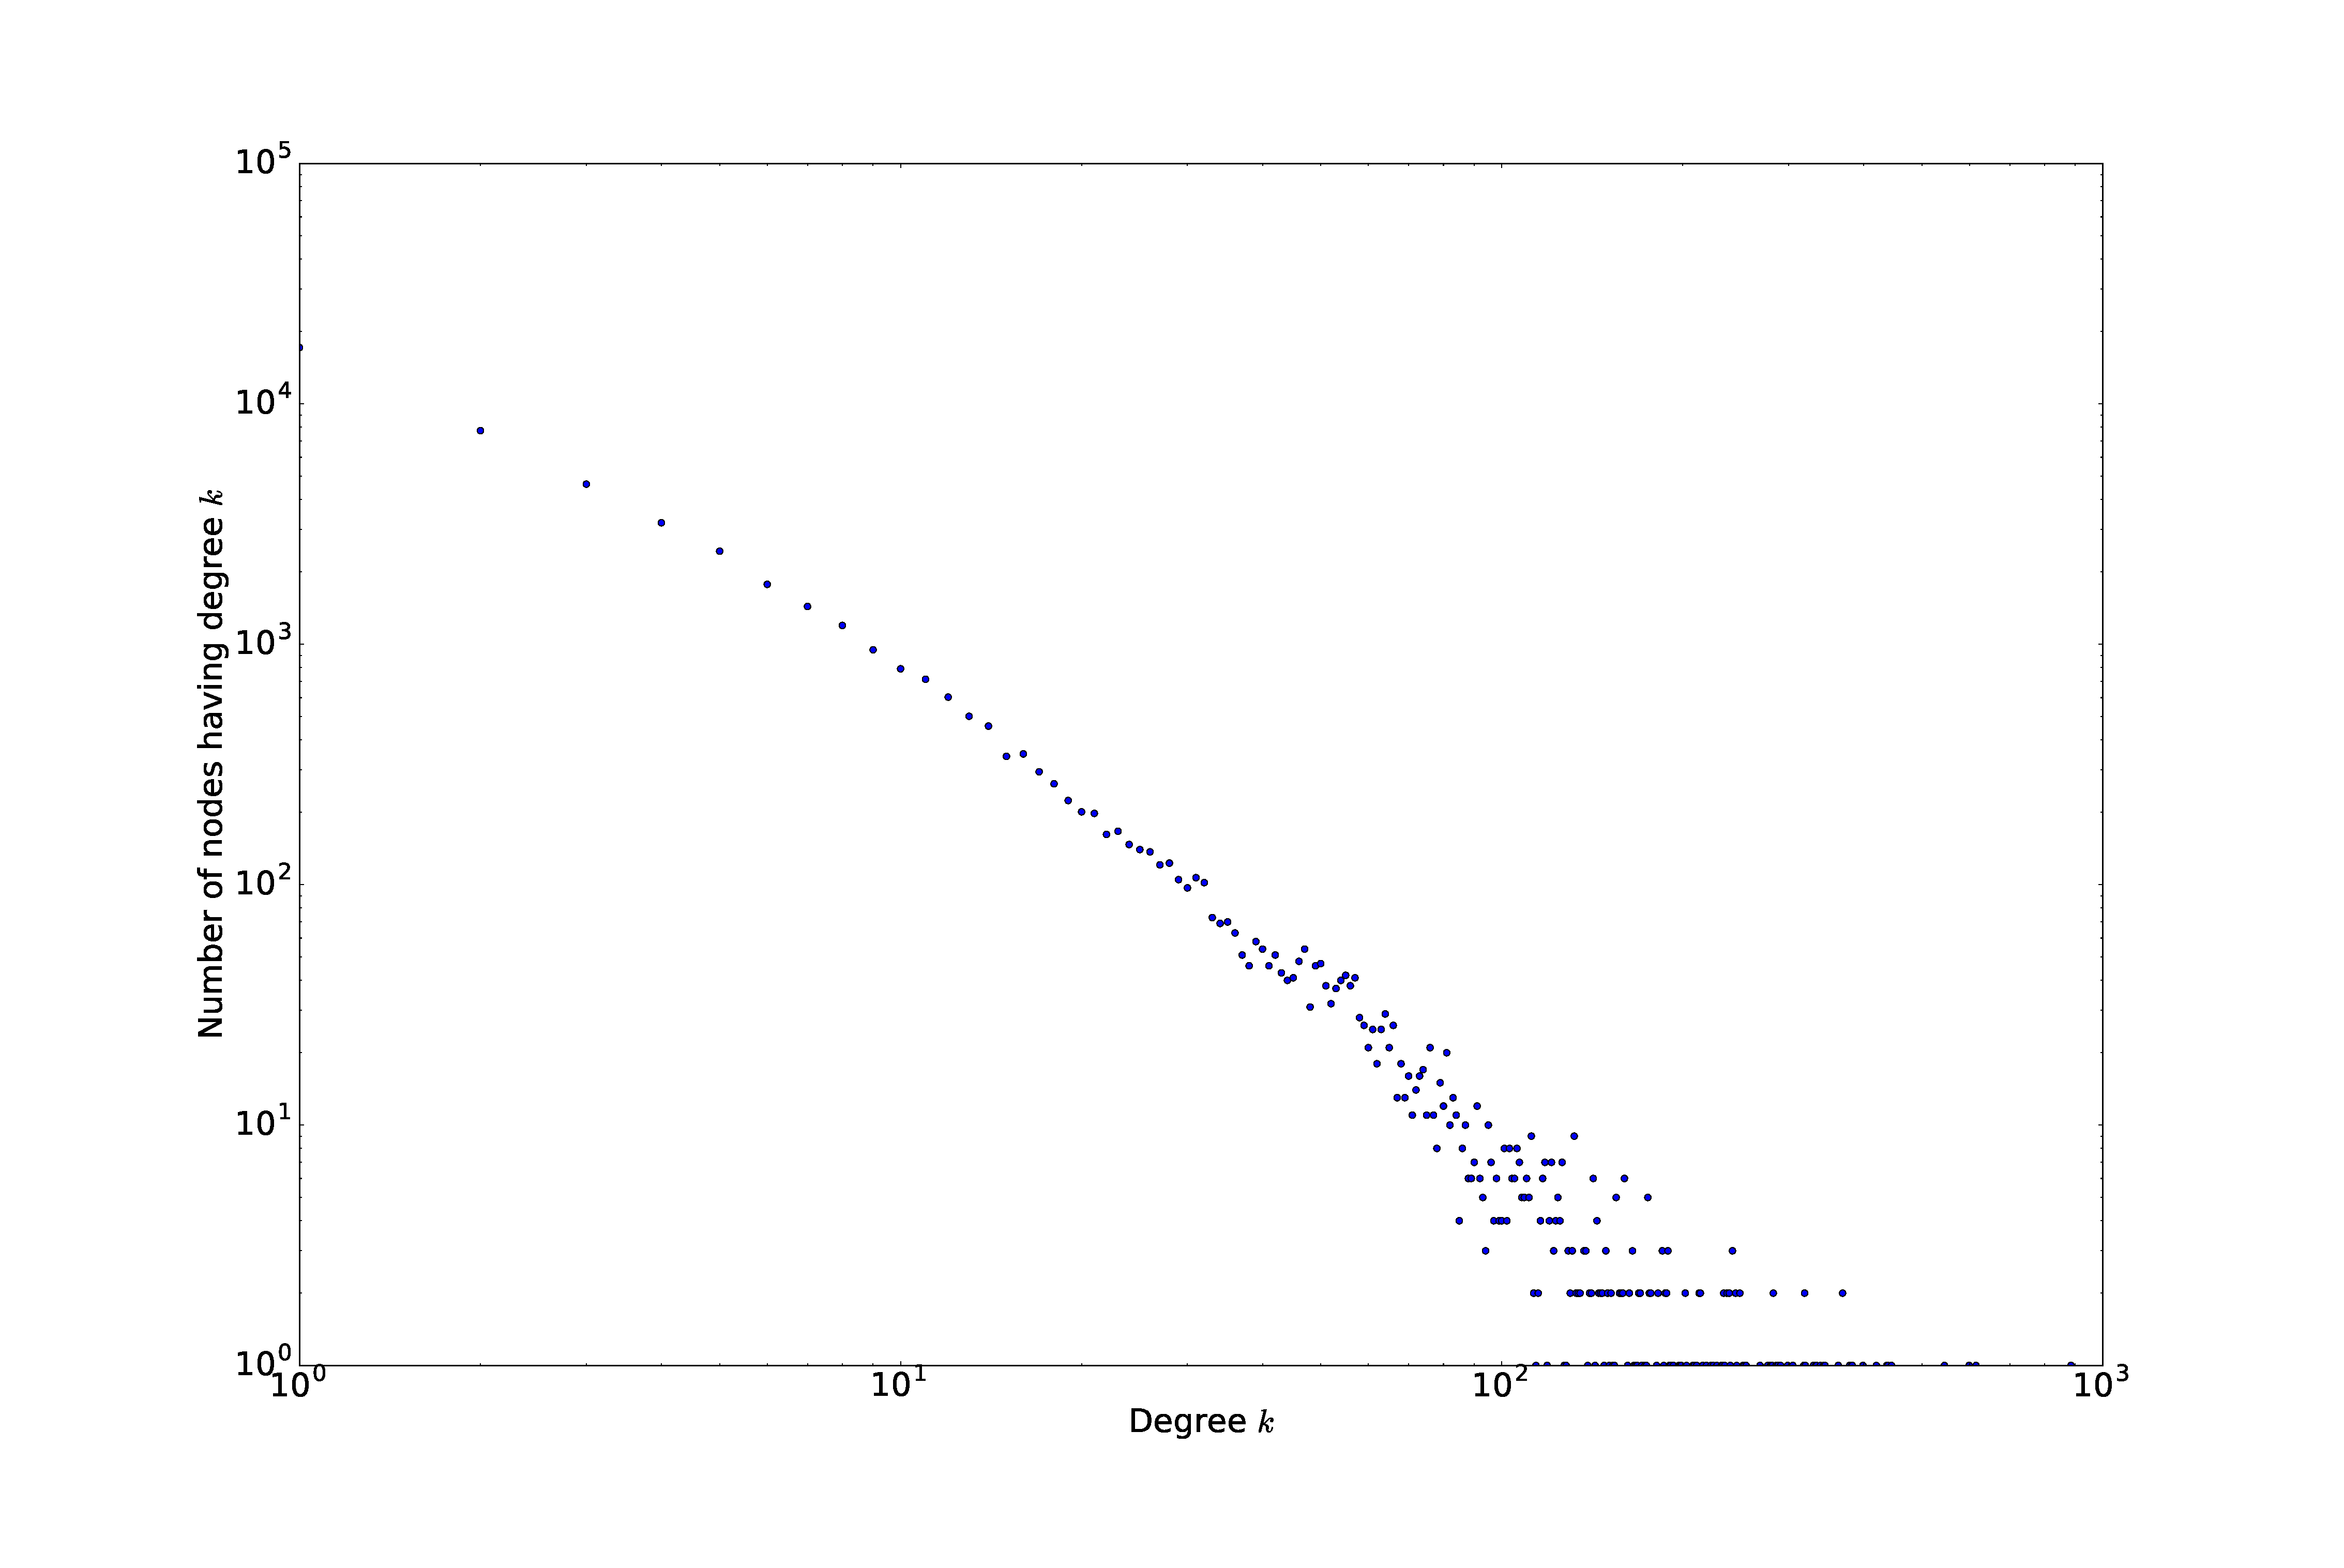
\includegraphics[width=100mm]{../fig/wot_degree_distribution.eps}}
      \caption{Web of Trustネットワークの次数分布}
      \label{fig:wot_dd}
     \end{figure}
  \subsection{シミュレーション結果}
   \subsubsection{未処理のネットワークに対する結果}
   図\ref{fig:succ_hops_full}, \ref{fig:cml_noclip}に未処理のネットワークに対するルーティングシミュレーション実験の結果を示す. 
   \begin{figure}[!h]
    \centerline{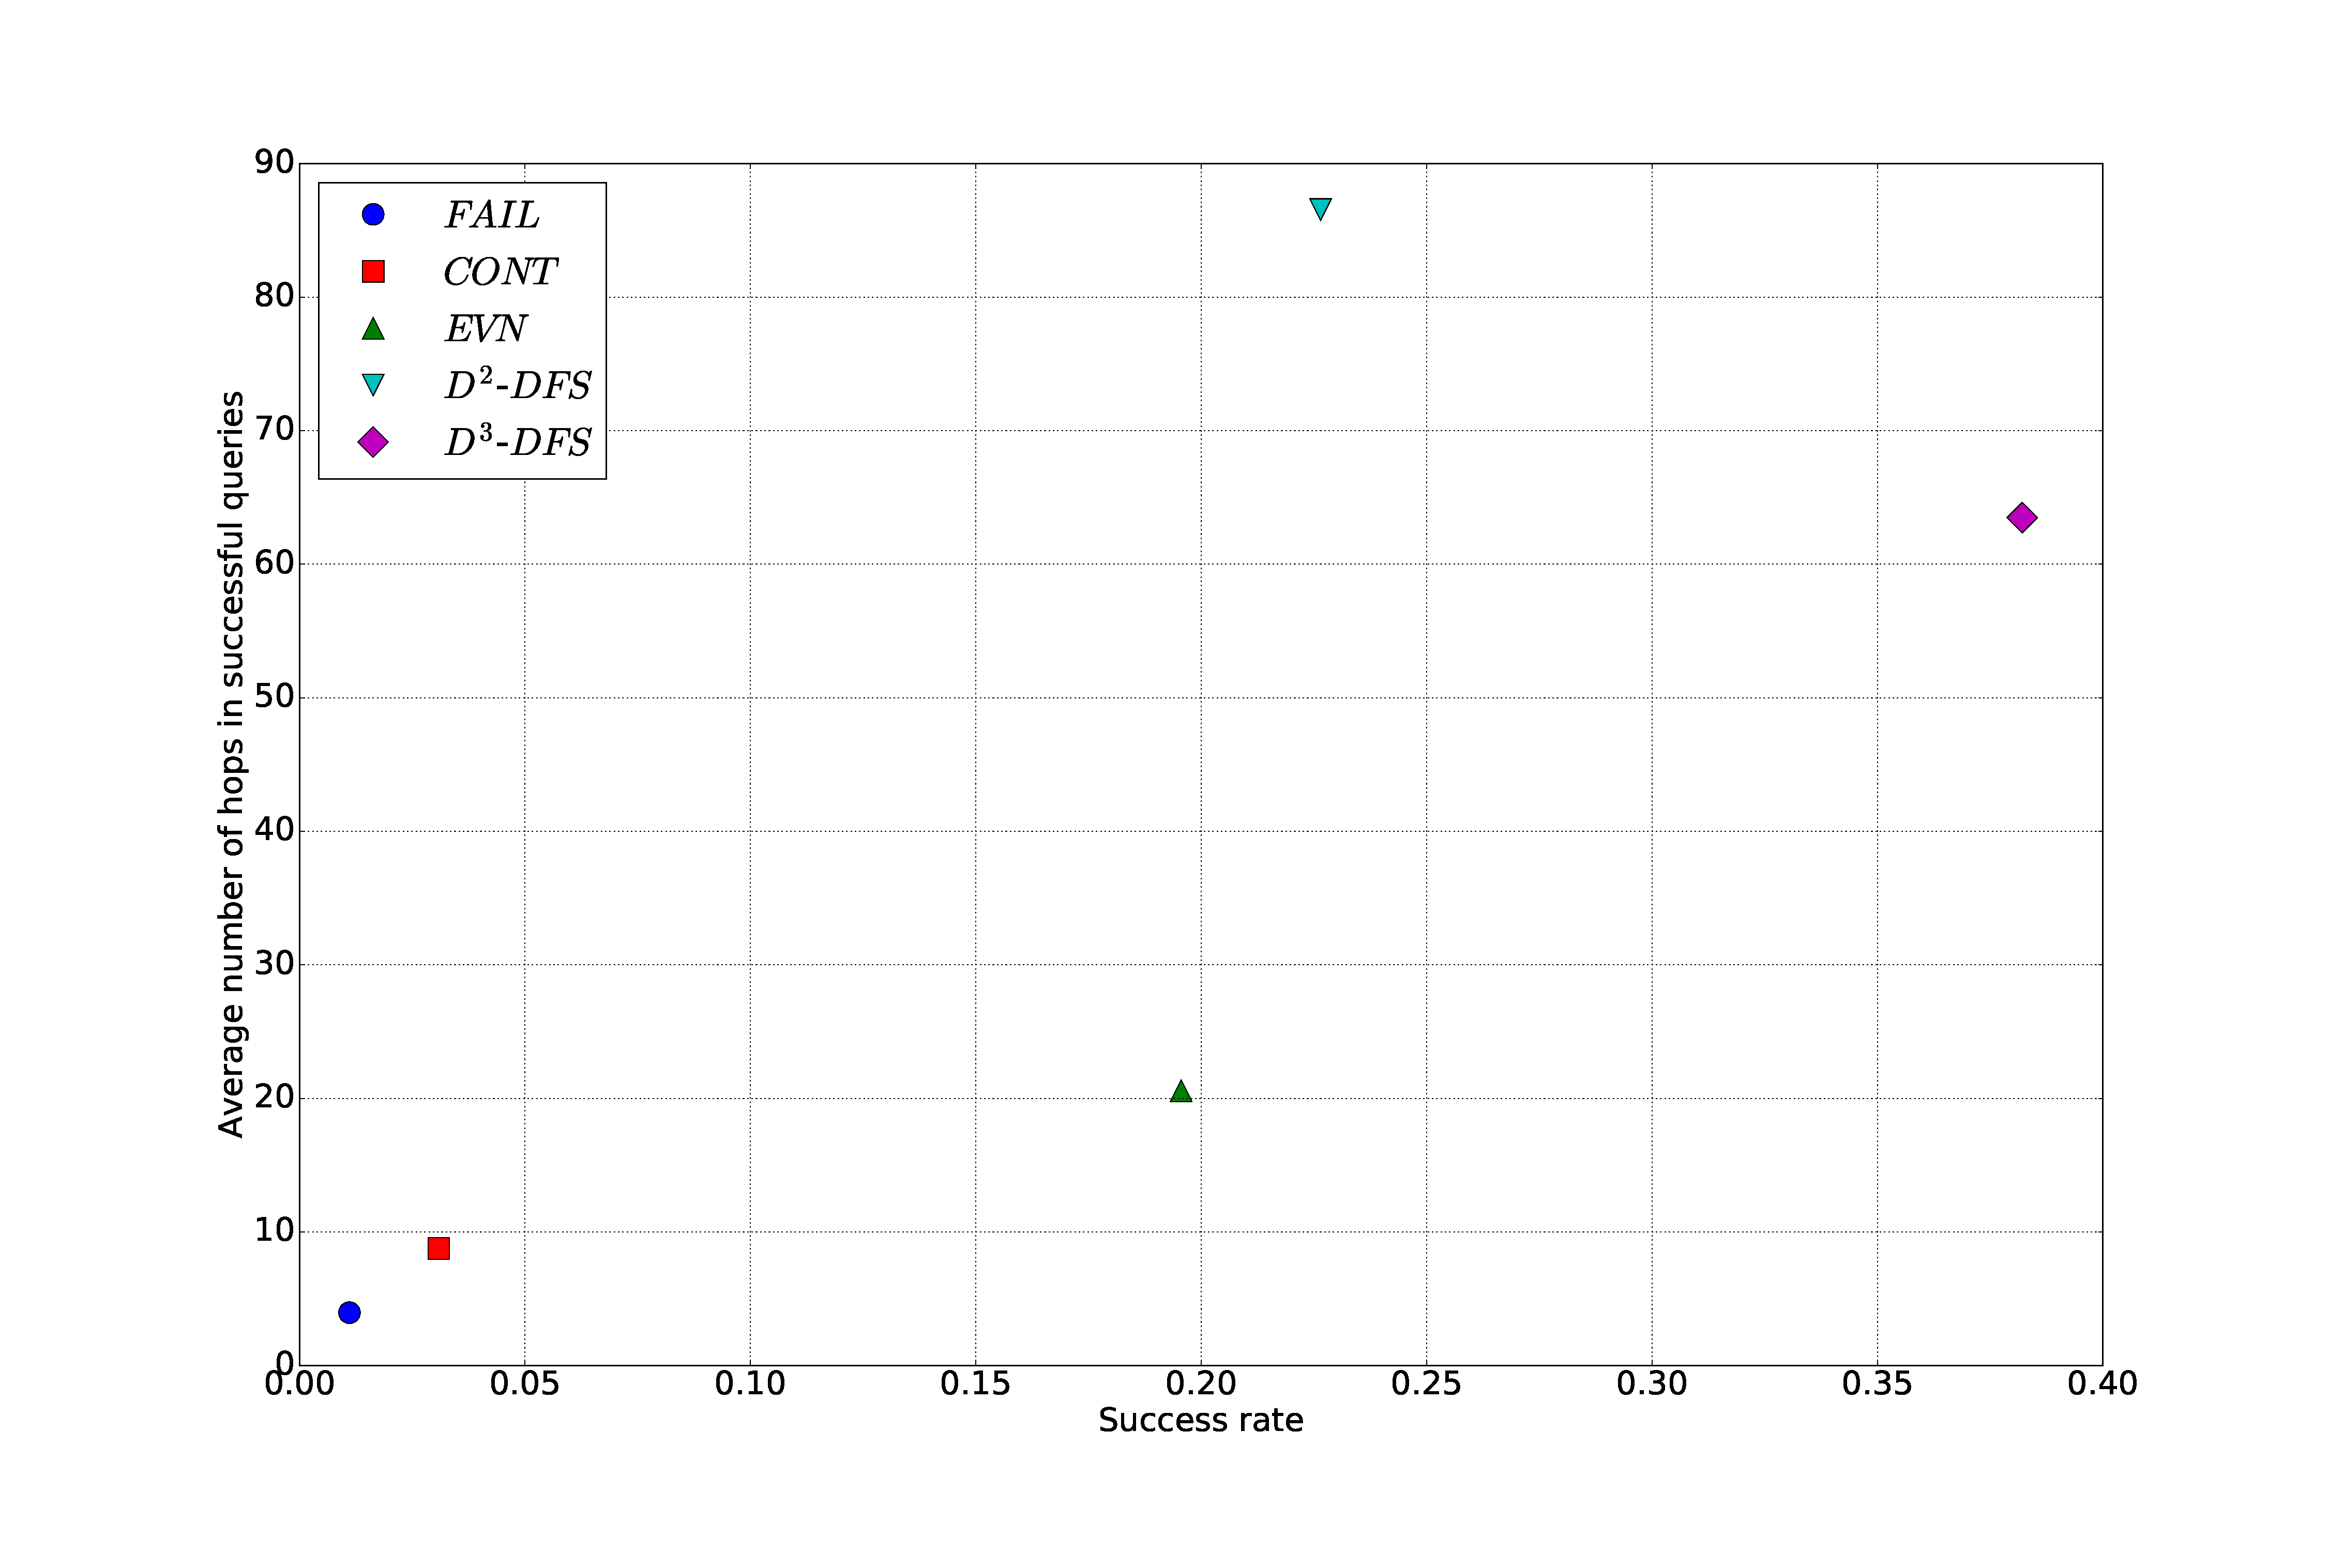
\includegraphics[width=100mm]{../fig/succ_hops_full.eps}}
    \caption{ID割り当て後のWeb of Trustネットワークにおける各ルーティングアルゴリズムの成功率と平均ホップ数}
    \label{fig:succ_hops_full}
   \end{figure}
   \begin{figure}[!h]
    \centerline{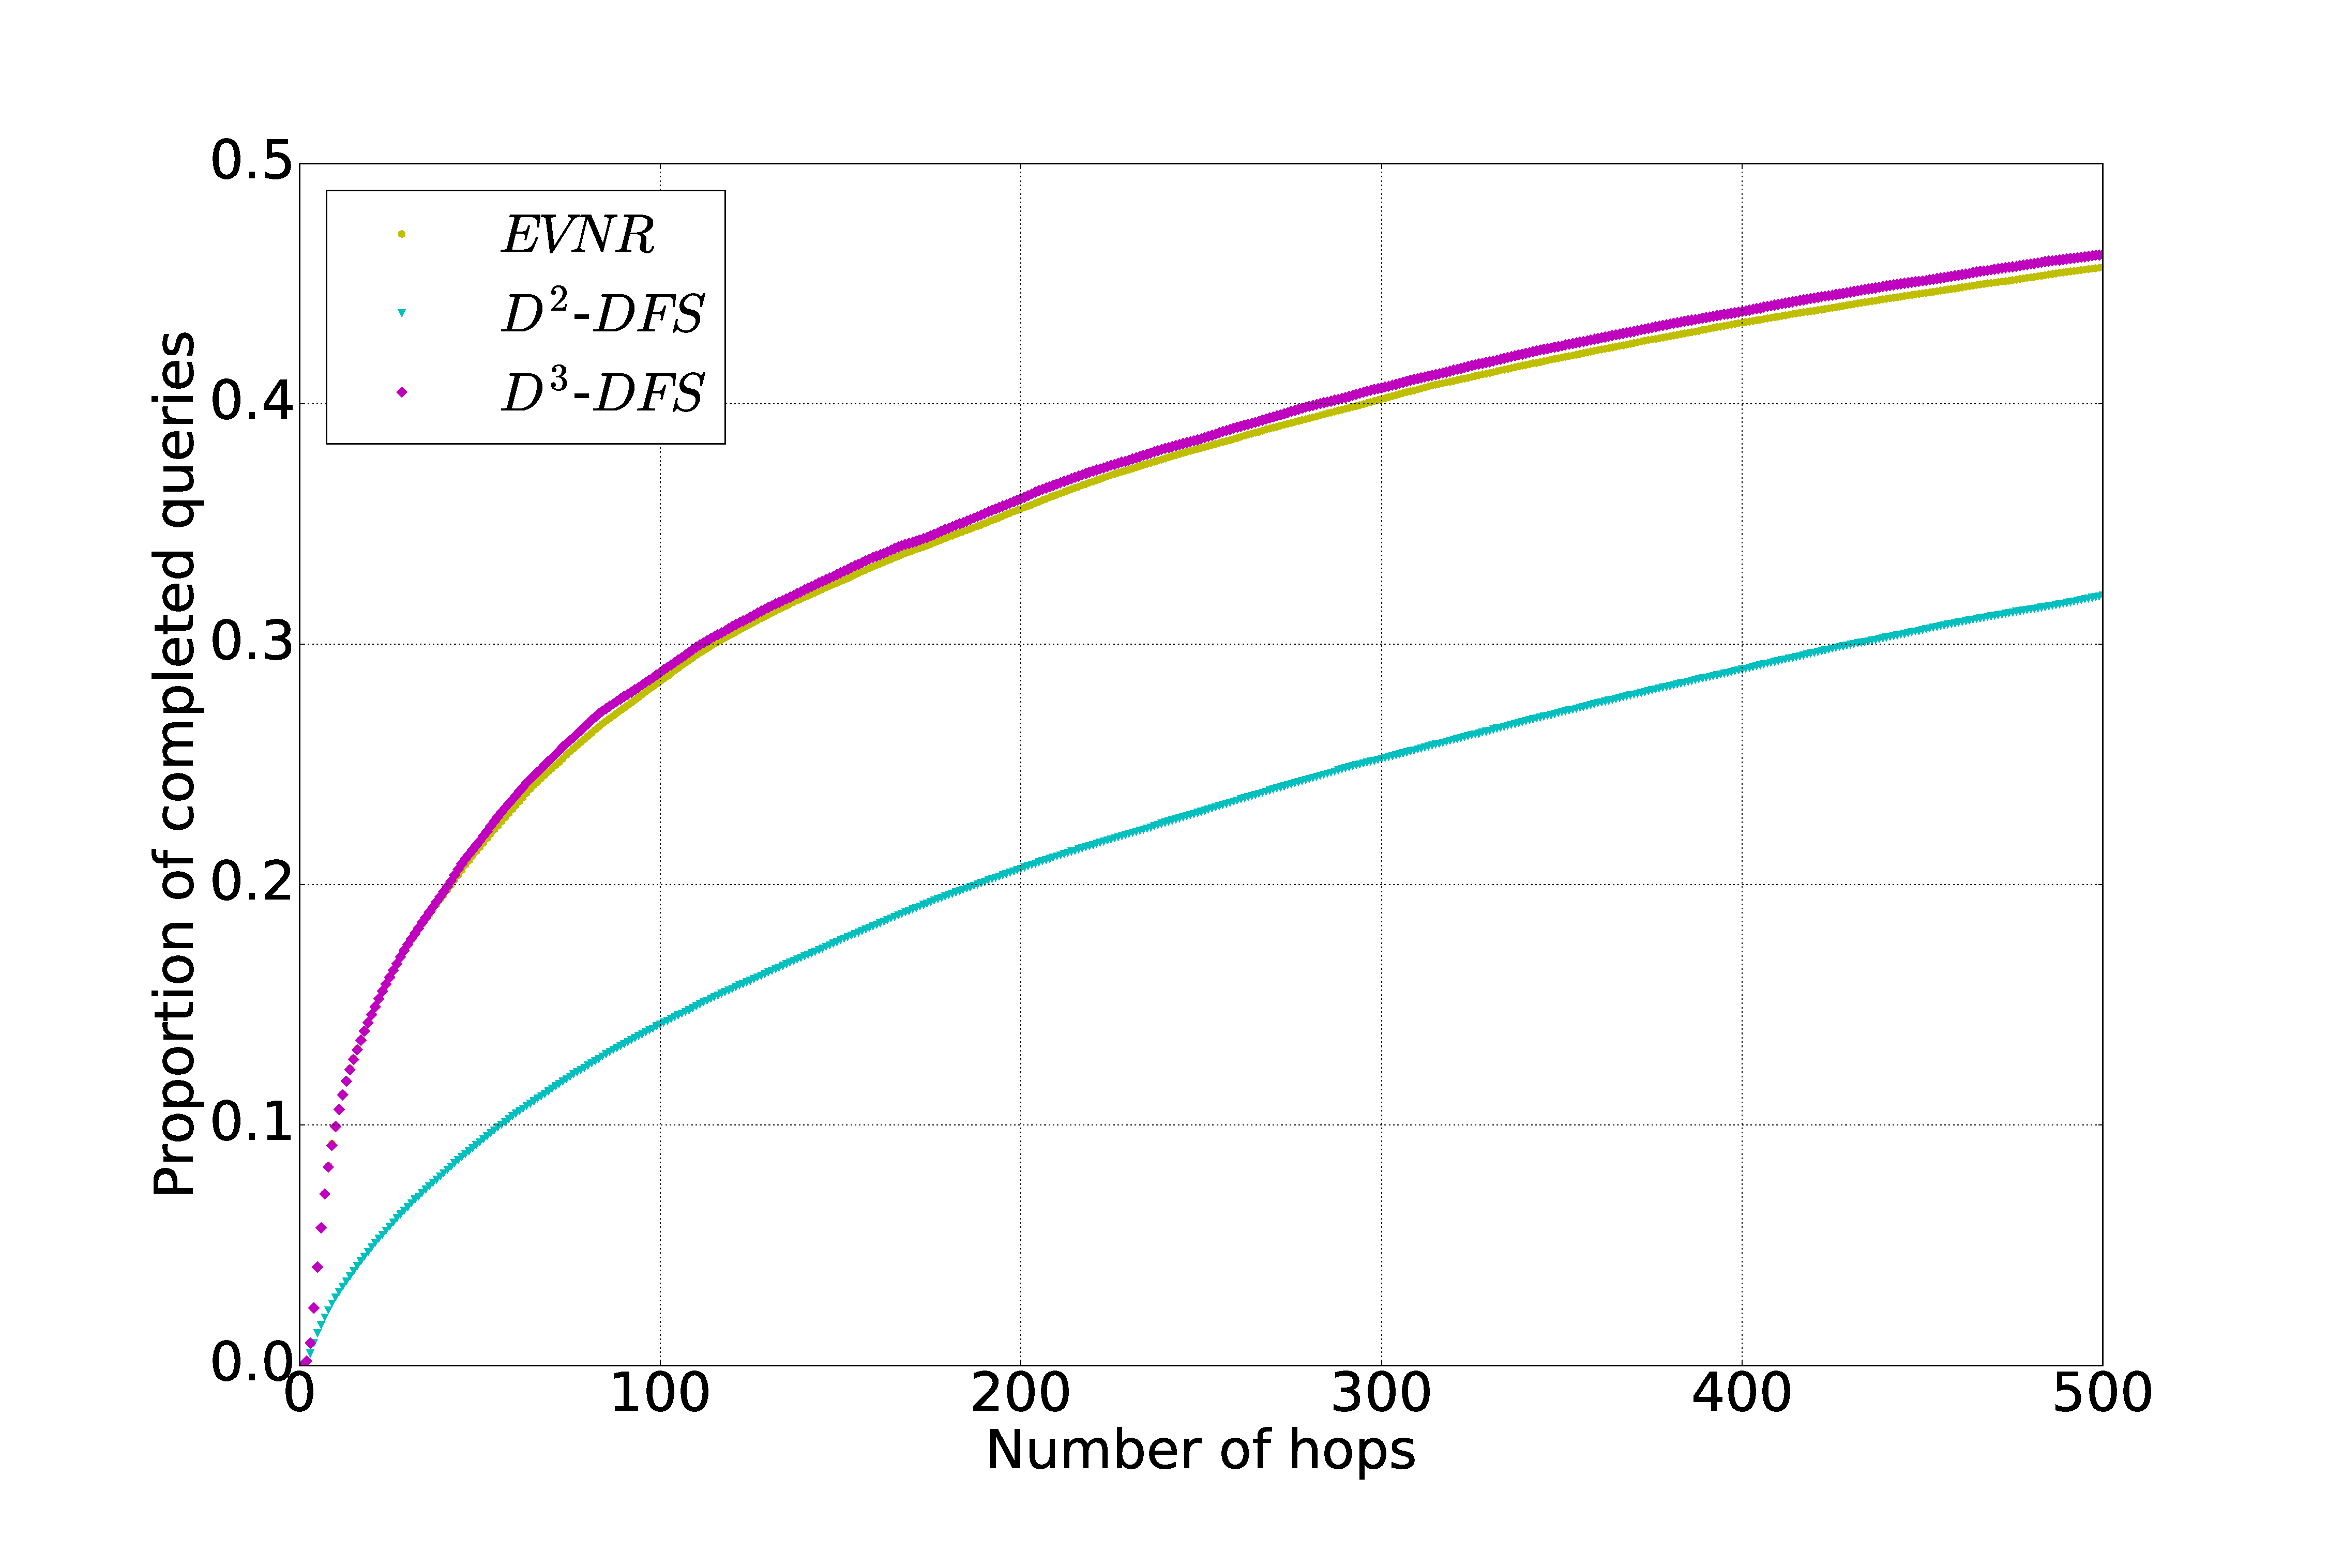
\includegraphics[width=100mm]{../fig/cml_noclip.eps}}
    \caption{ID割り当て後のWeb of Trustネットワークにおける各ホップ数以下で成功したルーティング試行の割合}
    \label{fig:cml_noclip}
   \end{figure}

   \subsubsection{次数上限を設けたネットワークに対する結果}
   \begin{figure}[!h]
    \centerline{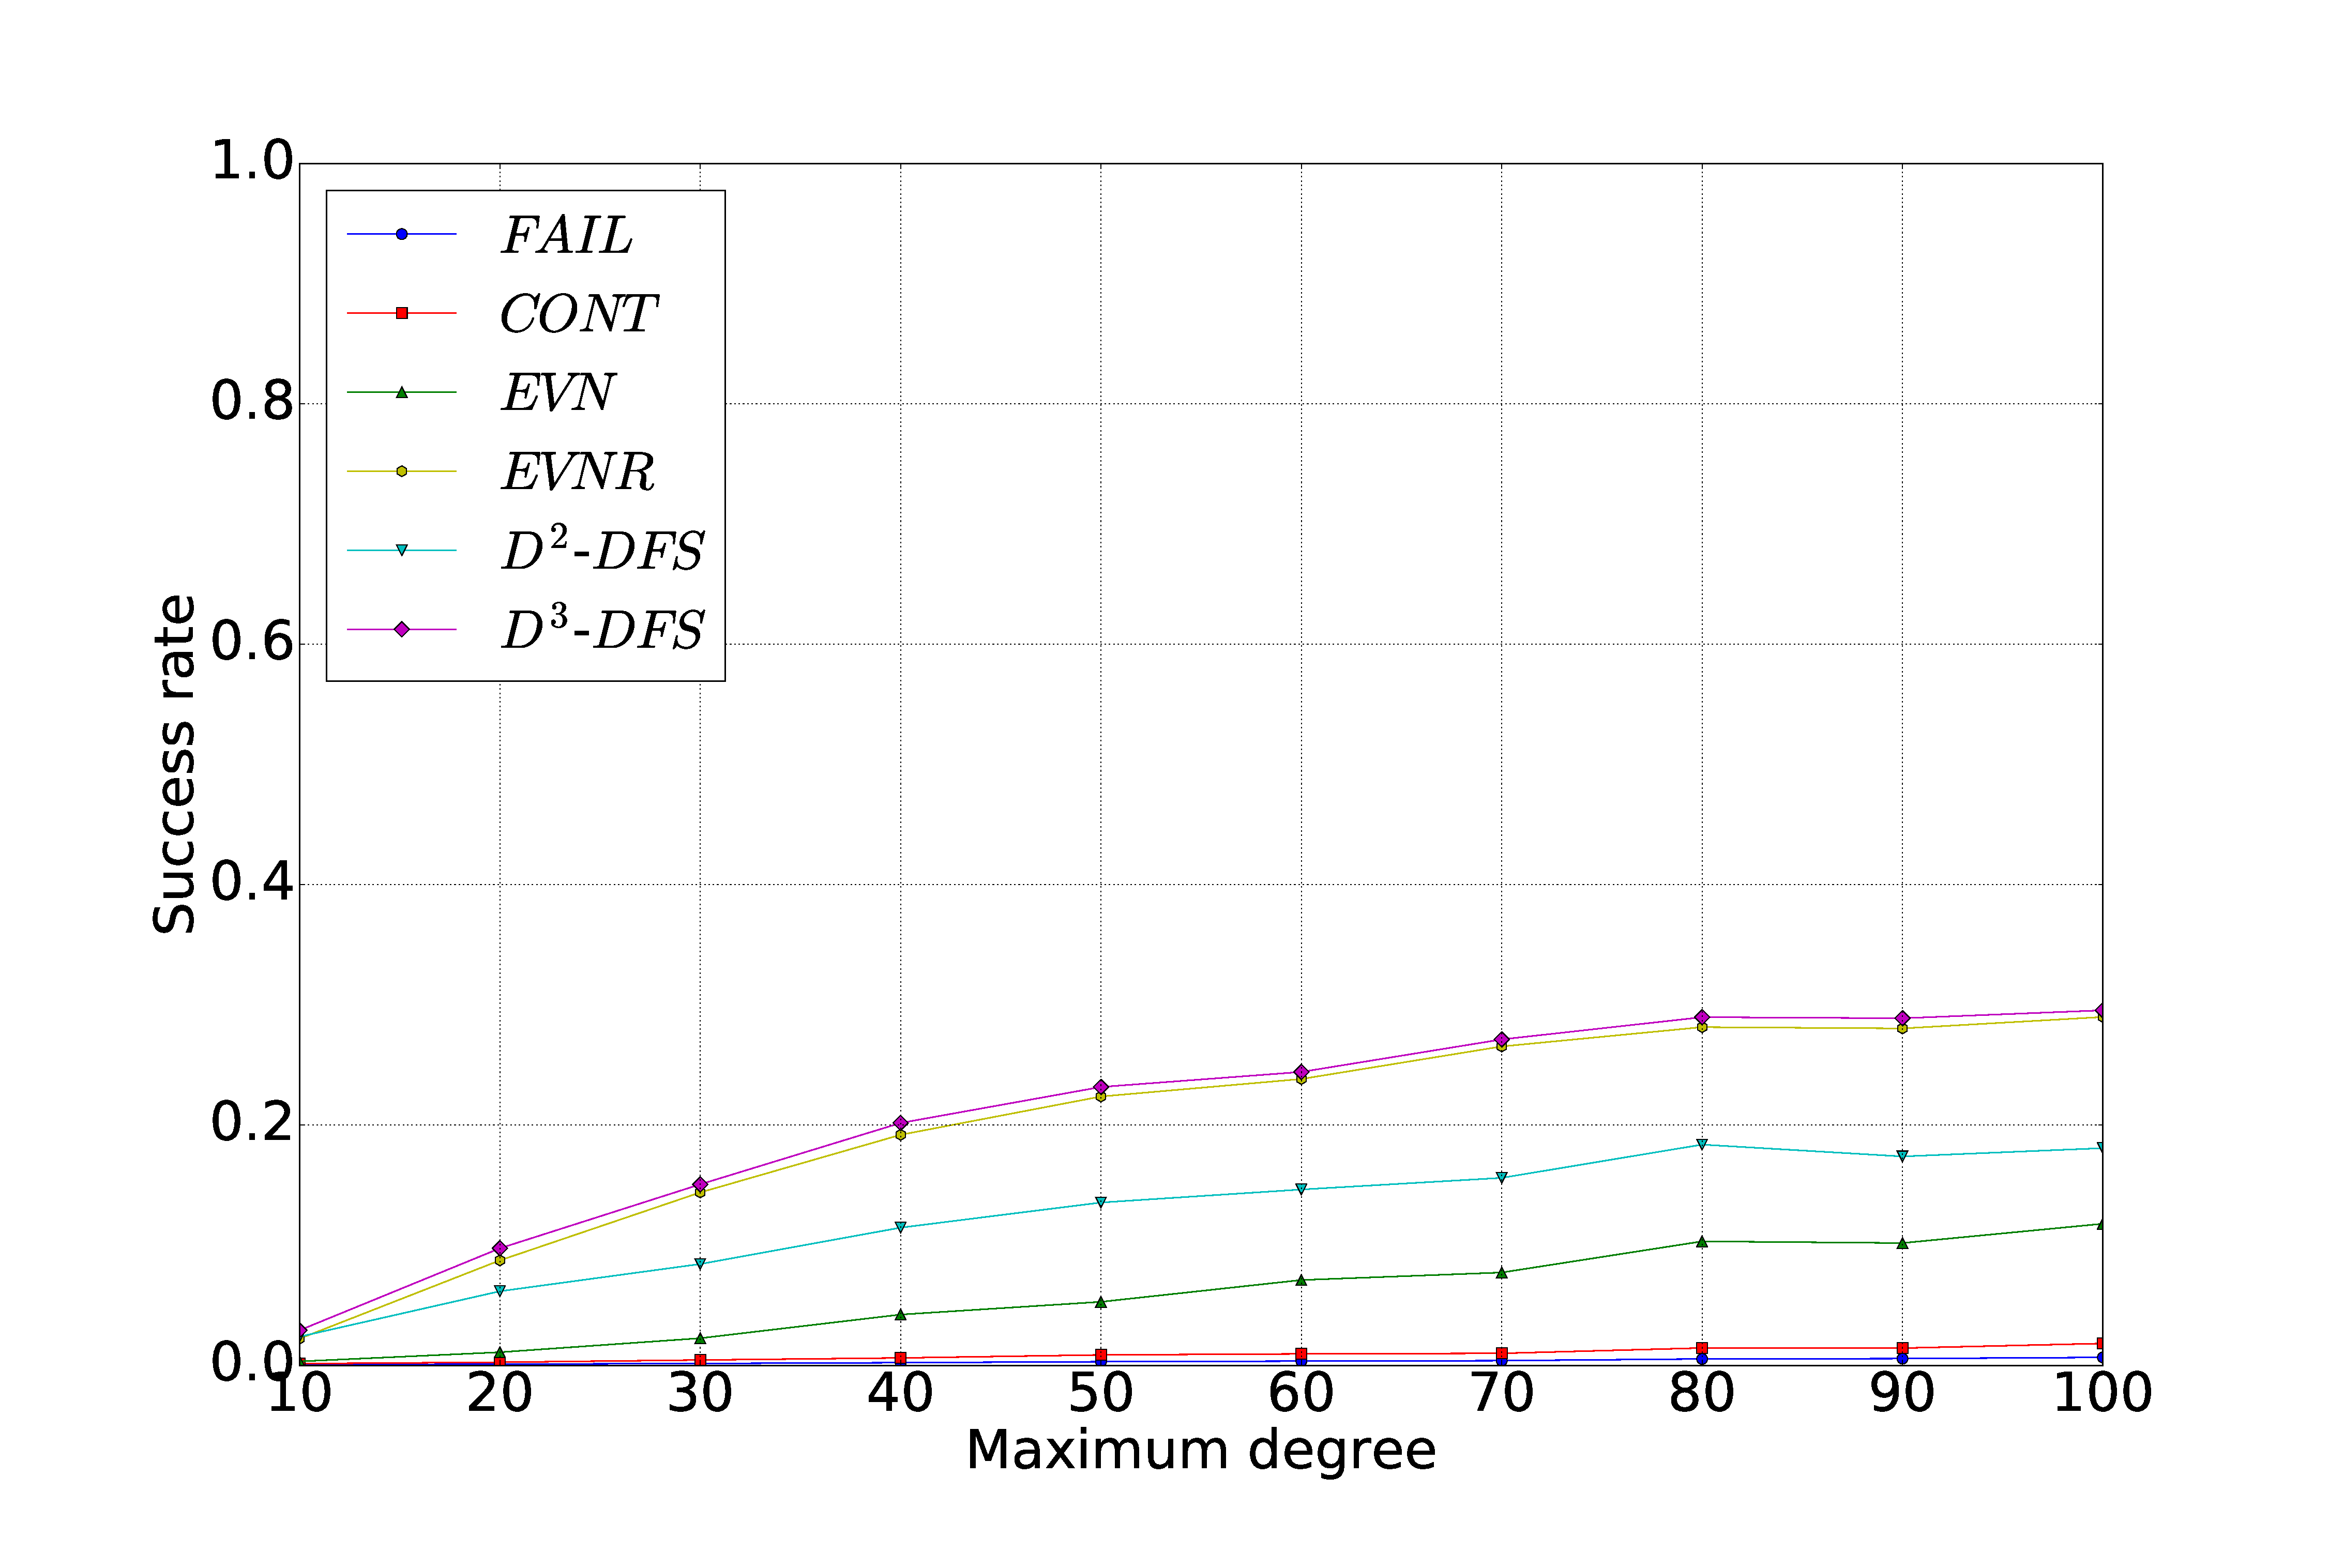
\includegraphics[width=100mm]{../fig/clip_succ.eps}}
    \caption{次数上限を設定したWeb of Trustネットワークにおける各ルーティングアルゴリズムの成功率}
    \label{fig:clip_succ}
   \end{figure}
   \begin{figure}[!h]
    \centerline{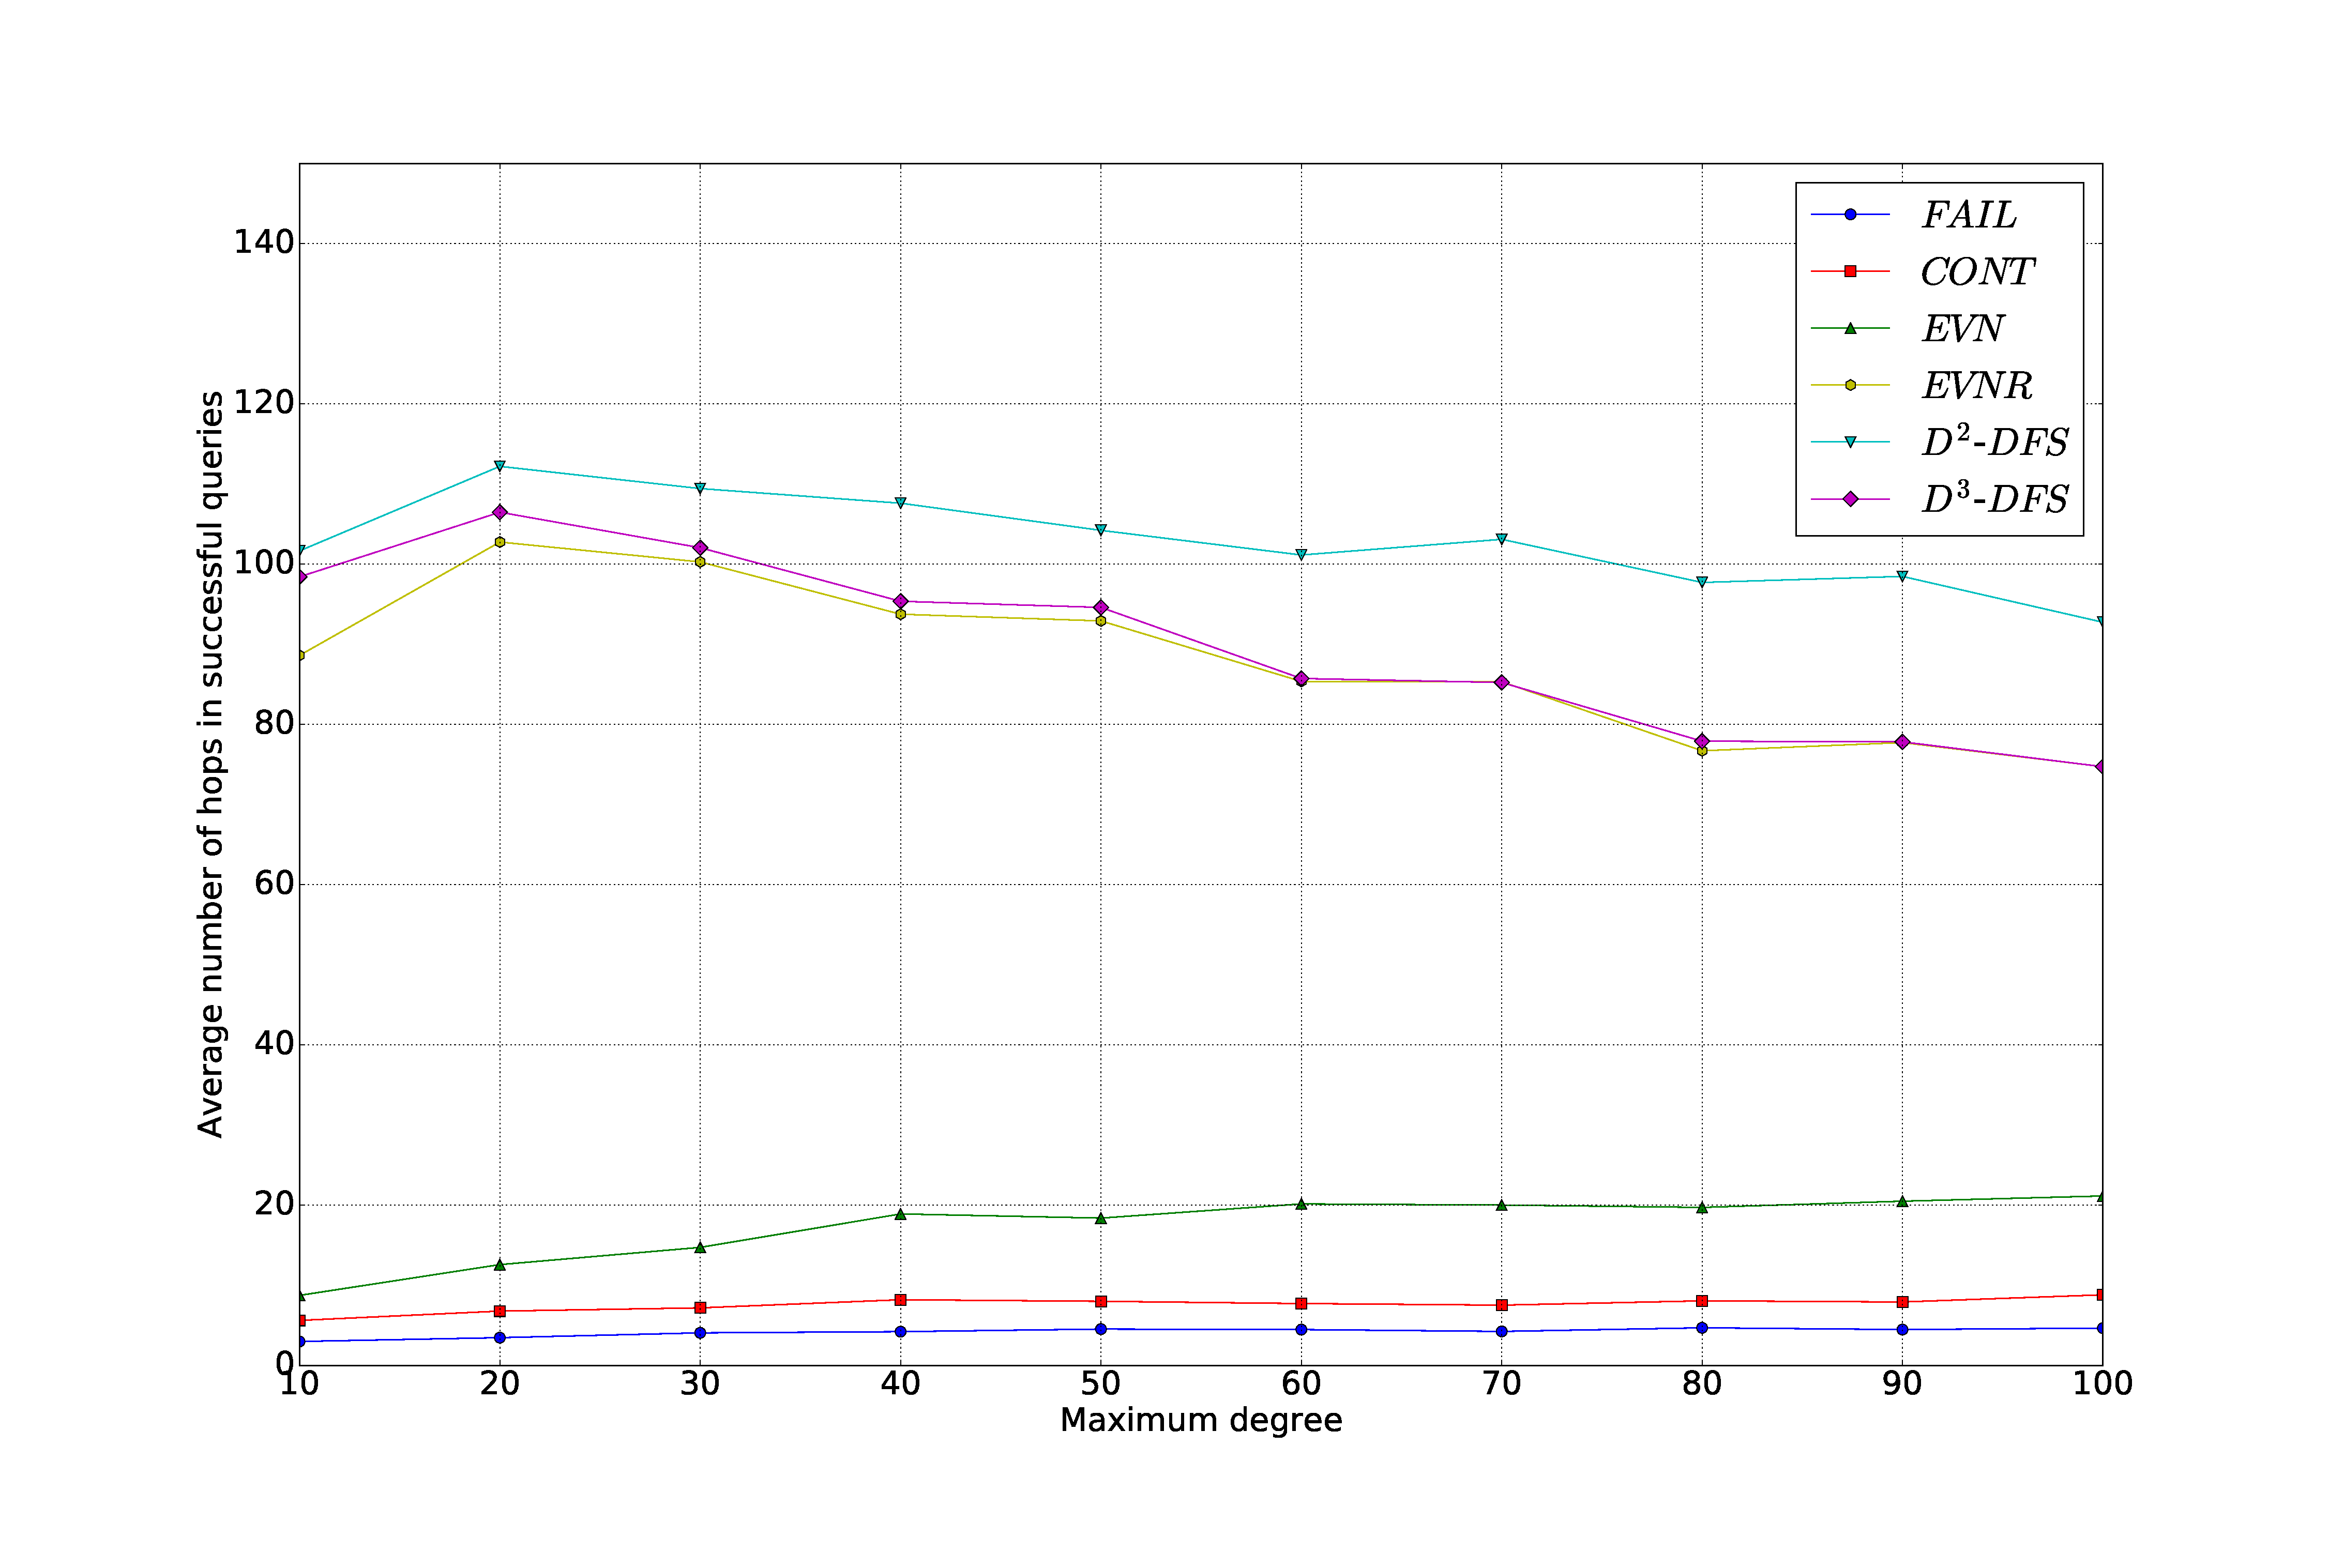
\includegraphics[width=100mm]{../fig/clip_hops.eps}}
    \caption{次数上限を設定したWeb of Trustネットワークにおける各ルーティングアルゴリズムの平均ホップ数}
    \label{fig:clip_hops}
   \end{figure}

\section{結論と今後の展望}
TBD
%% 謝辞 %%%%%%%%%%%%%%%%%%%%%%%%%%%%%%%%%%%%%%%%%%%%%%%%%%%%%%%%%%%%%%%%%%%%%%%%%
\acknowledgment
この場を借りて深く感謝を申し上げます.
%% 参考文献 %%%%%%%%%%%%%%%%%%%%%%%%%%%%%%%%%%%%%%%%%%%%%%%%%%%%%%%%%%%%%%%%%%%%%
\addcontentsline{toc}{section}{\refname} % 目次に参考文献を追加する.
                                         % chapter使用時は削除すること.

%% BibTeX 等を用いる場合は,上の thebibliography 環境を消してここに該当コードを
%% 挿入すること.
\bibliographystyle{ieeetr}
\bibliography{refs}


\clearpage
%% 付録 %%%%%%%%%%%%%%%%%%%%%%%%%%%%%%%%%%%%%%%%%%%%%%%%%%%%%%%%%%%%%%%%%%%%%%%%%
%% 付録は不要ならば削除してよい.
\appendix

\section{用語集}

\printglossaries


%% 本文ここまで %%%%%%%%%%%%%%%%%%%%%%%%%%%%%%%%%%%%%%%%%%%%%%%%%%%%%%%%%%%%%%%%%
\fi
\ifoutputcover
\evenclearpage
%% 表紙,背表紙,提出用摘要 %%%%%%%%%%%%%%%%%%%%%%%%%%%%%%%%%%%%%%%%%%%%%%%%%%%%%
\makecover                      % 表紙
\makespine[1]                   % 背表紙([] 内は出力枚数)
\makeinsidecover                % 中表紙
\fi
\ifoutputabstractforsubmission
\makeabstractforsubmission      % 提出用摘要
\fi
\end{document}
